\section{Finite State Automata}
{\tiny Every regular language is generated/recognized by an FSA, every FSA generates/recognizes a regular language\\
One of the states is the initial state, some states are accepting states\\
}\\
\scriptsize{Deterministic finite automata(DFA)} 
{\tiny At any state and for any input, a DFA has a single well-defined action to take\\
we can add a sink(or error) state to make all transitions well-defined (for brevity skipped)
}\\
\scriptsize{Non-deterministic finite automata(NFA)}\\ {\tiny transition table cells have sets of states\\
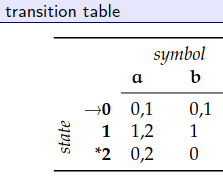
\includegraphics[scale=0.2]{transition-table.png}\\
NFA recognition(with backtracking)\\
1. start at q0\\
2. take the next input, place all possible actions to an agenda (state, character index)\\
3. get the next action from the agenda, act\\
4. at the end of input: accept-if in an accepting state; reject-not in accepting state \& agenda empty; backtrack-otherwise\\
worst time complexity is exponential\\
depth-first search with stack as agenda, breath-first search with queue as agenda\\
machine learning methods to guide a best solution\\
NFA recognition(parallel version)\
1. start at q0\\
2. take the next input, mark all possible next states\\
3. if an accepting state is marked at the end of the input, accept\\
note: the process is deterministic and finite-state\\
}\\
\scriptsize{$\epsilon$-NFA} {\tiny allows moving without consuming an input symbol\\
any $\epsilon$-NFA can be converted to an NFA\\
}\\
\scriptsize{NFA-DFA equivalence}\\
{\tiny the set of DFA is a subset of the set of NFA(DFA is also an NFA)\\
NFA can automatically be converted to the equivalent DFA\\
DFA recognition is O(n), NFA recognition may be exponential\\
NFA are often easier to construct/may require less memory
}\\
\scriptsize{$\epsilon$ removal}\\ 
{\tiny 1. start with finding the $\epsilon$-closure of all states\\
2. replace each arc to each state with arc(s) to all states in the $\epsilon$-closure\\
with transition table:\\
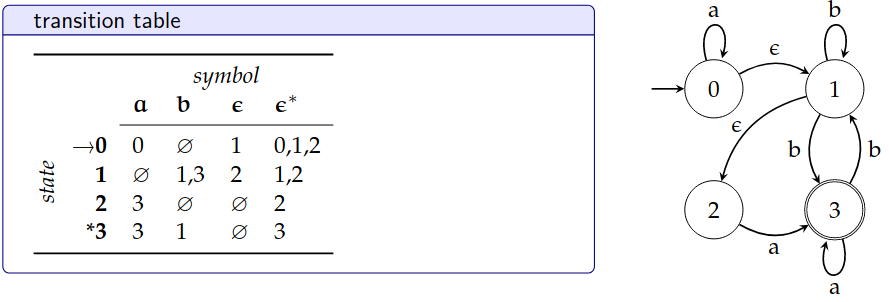
\includegraphics[scale=0.15]{epsilon-removal.png}\\
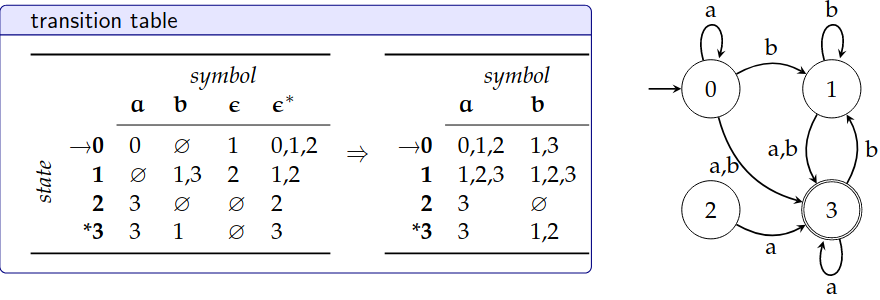
\includegraphics[scale=0.15]{epsilon-removal1.png}
}
\subsection*{NFA Determinization}
\scriptsize{subset construction}\\
{\tiny 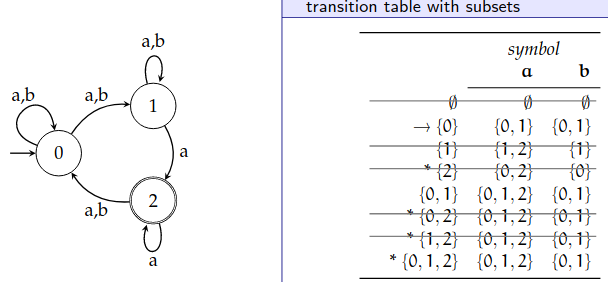
\includegraphics[scale=0.2]{subset-construction.png}\\
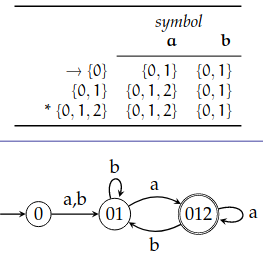
\includegraphics[scale=0.2]{subset-construction1.png}\\
can skip the unreachable states during subset construction
}
\subsection*{FSA Minimization}
{\tiny for any regular language there is a unique minimal DFA\\
throw away unreachable states, merge equivalent states
}\\
\scriptsize{Hopcroft's algorithm}
{\tiny find and eliminate equivalent states by partitioning the set of states\\
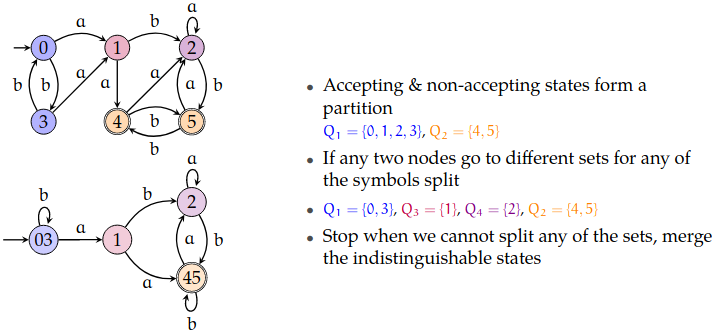
\includegraphics[scale=0.2]{partitioning.png}\\
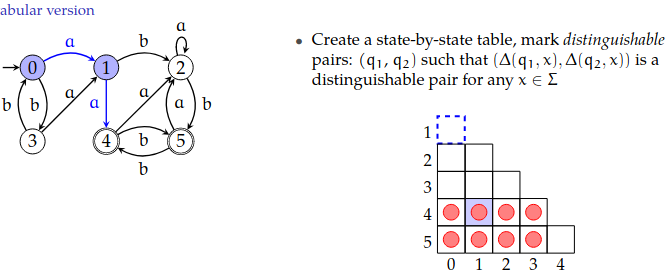
\includegraphics[scale=0.2]{partitioning-tabular.png}\\
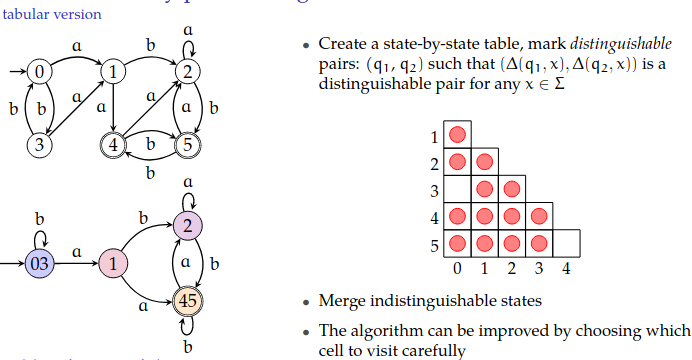
\includegraphics[scale=0.2]{partitioning-tabular1.png}\\
O(n log n) complexity
}\\
\scriptsize{Brzozowski’s algorithm} {\tiny 'double reversal'\\
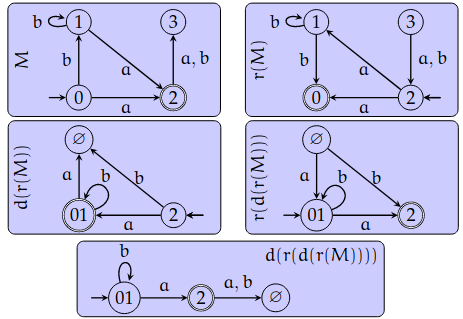
\includegraphics[scale=0.2]{brzozowski.png}\\
exponential worst-time complexity\\
can also be used with NFAs(resulting in the minimal equivalent DFA)
}
\subsection*{Finite State Transducers}
{\tiny The machine moves between the states based on an input symbol, while it outputs the corresponding output symbol\\
The relation defined by an FST is called a regular (or rational) relation\\
we treat an FSA as a simple FST that outputs its input\\
FST share many properties of FSAs, however:\\
- FSTs are not closed under intersection and complement\\
- we can compose(and invert) FSTs\\
- determinizing FSTs is not always possible
}\\
\scriptsize{FST inversion (M**-1)}\\
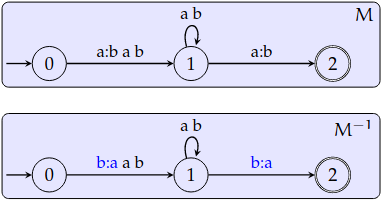
\includegraphics[scale=0.2]{fst-inversion.png}\\
\scriptsize{FST composition}\\ {\tiny sequential application:\\ 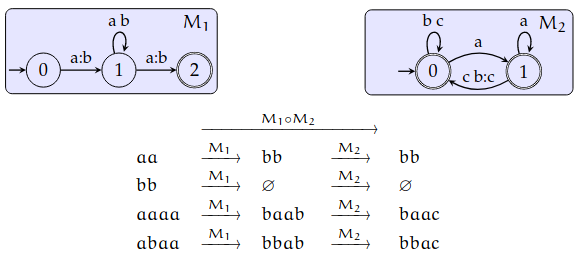
\includegraphics[scale=0.2]{fst-composition.png}\\
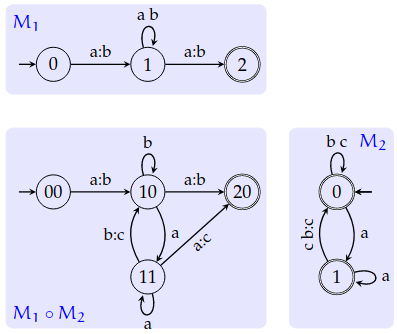
\includegraphics[scale=0.2]{fst-composition1.png}
}\\
\scriptsize{FST projection} {\tiny
turns an FST into a FSA, accepting either the input language or the output language\\
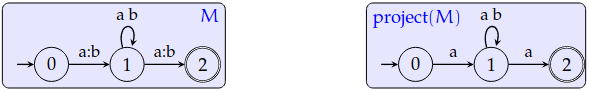
\includegraphics[scale=0.2]{fst-projection.png}
}\\
\scriptsize{FST determinization} {\tiny
means converting to a subsequential FST\\
can extend the subset construction to FSTs\\
not all FSTs can be determinized\\
}\\
\scriptsize{sequential FSTs} {\tiny
has a single transition from each state on every input symbol\\
Output symbols can be strings, as well as $\epsilon$\\
linear recognition time\\
do not allow ambiguity\\
}\\
\scriptsize{subsequential FSTs} {\tiny
A k-subsequential FST is a sequential FST which can output up to k strings at an accepting state\\
allow limited ambiguity\\
linear recognition time\\
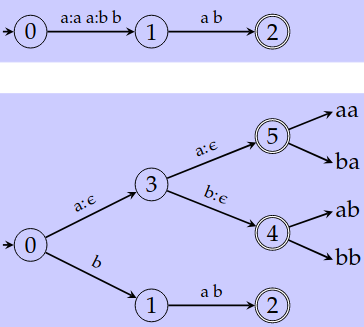
\includegraphics[scale=0.2]{fst-determinization.png}
}\\